% !TeX spellcheck = en_US
\documentclass{beamer}
\usepackage{ctex, hyperref}
\usepackage[T1]{fontenc}

% other packages
\usepackage{latexsym,amsmath,xcolor,multicol,booktabs,calligra, tikz}
\usepackage{graphicx,pstricks,listings,stackengine}

\author{Axel Fritz, You Ming}
\title{Project Proposal}
\subtitle{Numerical Simulation of Manufacturing Processes}
\institute{Dept. of Mechanical Engineering}
\date{April 20, 2026}
\usepackage{Tsinghua}

% defs
\def\cmd#1{\texttt{\color{red}\footnotesize $\backslash$#1}}
\def\env#1{\texttt{\color{blue}\footnotesize #1}}
\definecolor{deepblue}{rgb}{0,0,0.5}
\definecolor{deepred}{rgb}{0.6,0,0}
\definecolor{deepgreen}{rgb}{0,0.5,0}
\definecolor{halfgray}{gray}{0.55}

\lstset{
	basicstyle=\ttfamily\small,
	keywordstyle=\bfseries\color{deepblue},
	emphstyle=\ttfamily\color{deepred},    % Custom highlighting style
	stringstyle=\color{deepgreen},
	numbers=left,
	numberstyle=\small\color{halfgray},
	rulesepcolor=\color{red!20!green!20!blue!20},
	frame=shadowbox,
}


\begin{document}
	
	\kaishu
	\begin{frame}
		\titlepage
		\begin{figure}[htpb]
			\begin{center}
				
\includegraphics[width=0.2\linewidth]{pic/Tsinghua_University_Logo.eps}
			\end{center}
		\end{figure}
	\end{frame}
	
	\begin{frame}
		\tableofcontents[sectionstyle=show,subsectionstyle=show/shaded/hide,subsubsectionstyle=show/shaded/hide]
	\end{frame}

	\section{Background}
	\subsection{TPMS}
	\begin{frame}{Triply Periodic Minimal Surface (TPMS)}
		TMPS are surfaces with the following mathematical properties \cite{enwiki:TPMS}:
		\begin{itemize}
			\item Nearly all studied TPMS are free of self-intersections (i.e. embedded in $\mathbb{R}^3$).
			\item All connected TPMS have genus $\geq 3$, and in every lattice there exist orientable embedded TPMS of every genus $\geq 3$.
			\item Embedded TPMS are orientable and divide space into two disjoint sub-volumes (labyrinths).
		 \end{itemize}
		 The mathematical background of TPMS is not particularly relevant for this project, but we will make use of the last property. 
	\end{frame}
	\begin{frame}{Gyroid-TPMS}
		Discovered by NASA scientist Alan Schoen in 1970, proved to be embedded by Grosse-Brauckmann and Wohlgemuth in 1996 \cite{enwiki:gyroid}. It is the structure that we will be treating in this project. 
		\begin{itemize}
			\item Embedded; divides space into two \emph{disjoint} sub-volumes. 
			\item Can be approximated a the relatively simple equation
			\begin{equation*}
				\sin x\cos y+\sin y\cos z+\sin z\cos x=0
			\end{equation*}
		\end{itemize}
		\centering
		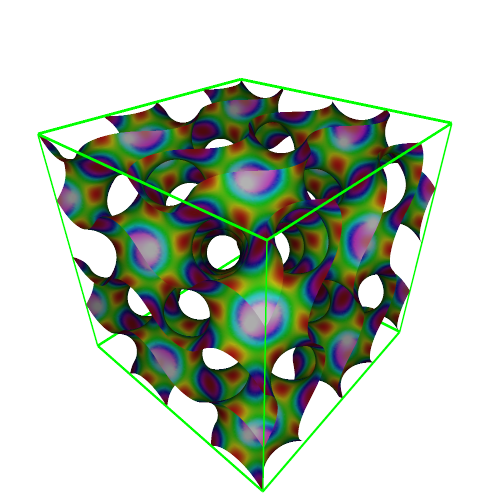
\includegraphics[scale=0.2]{pic/Gyroid_surface_with_Gaussian_curvature}
		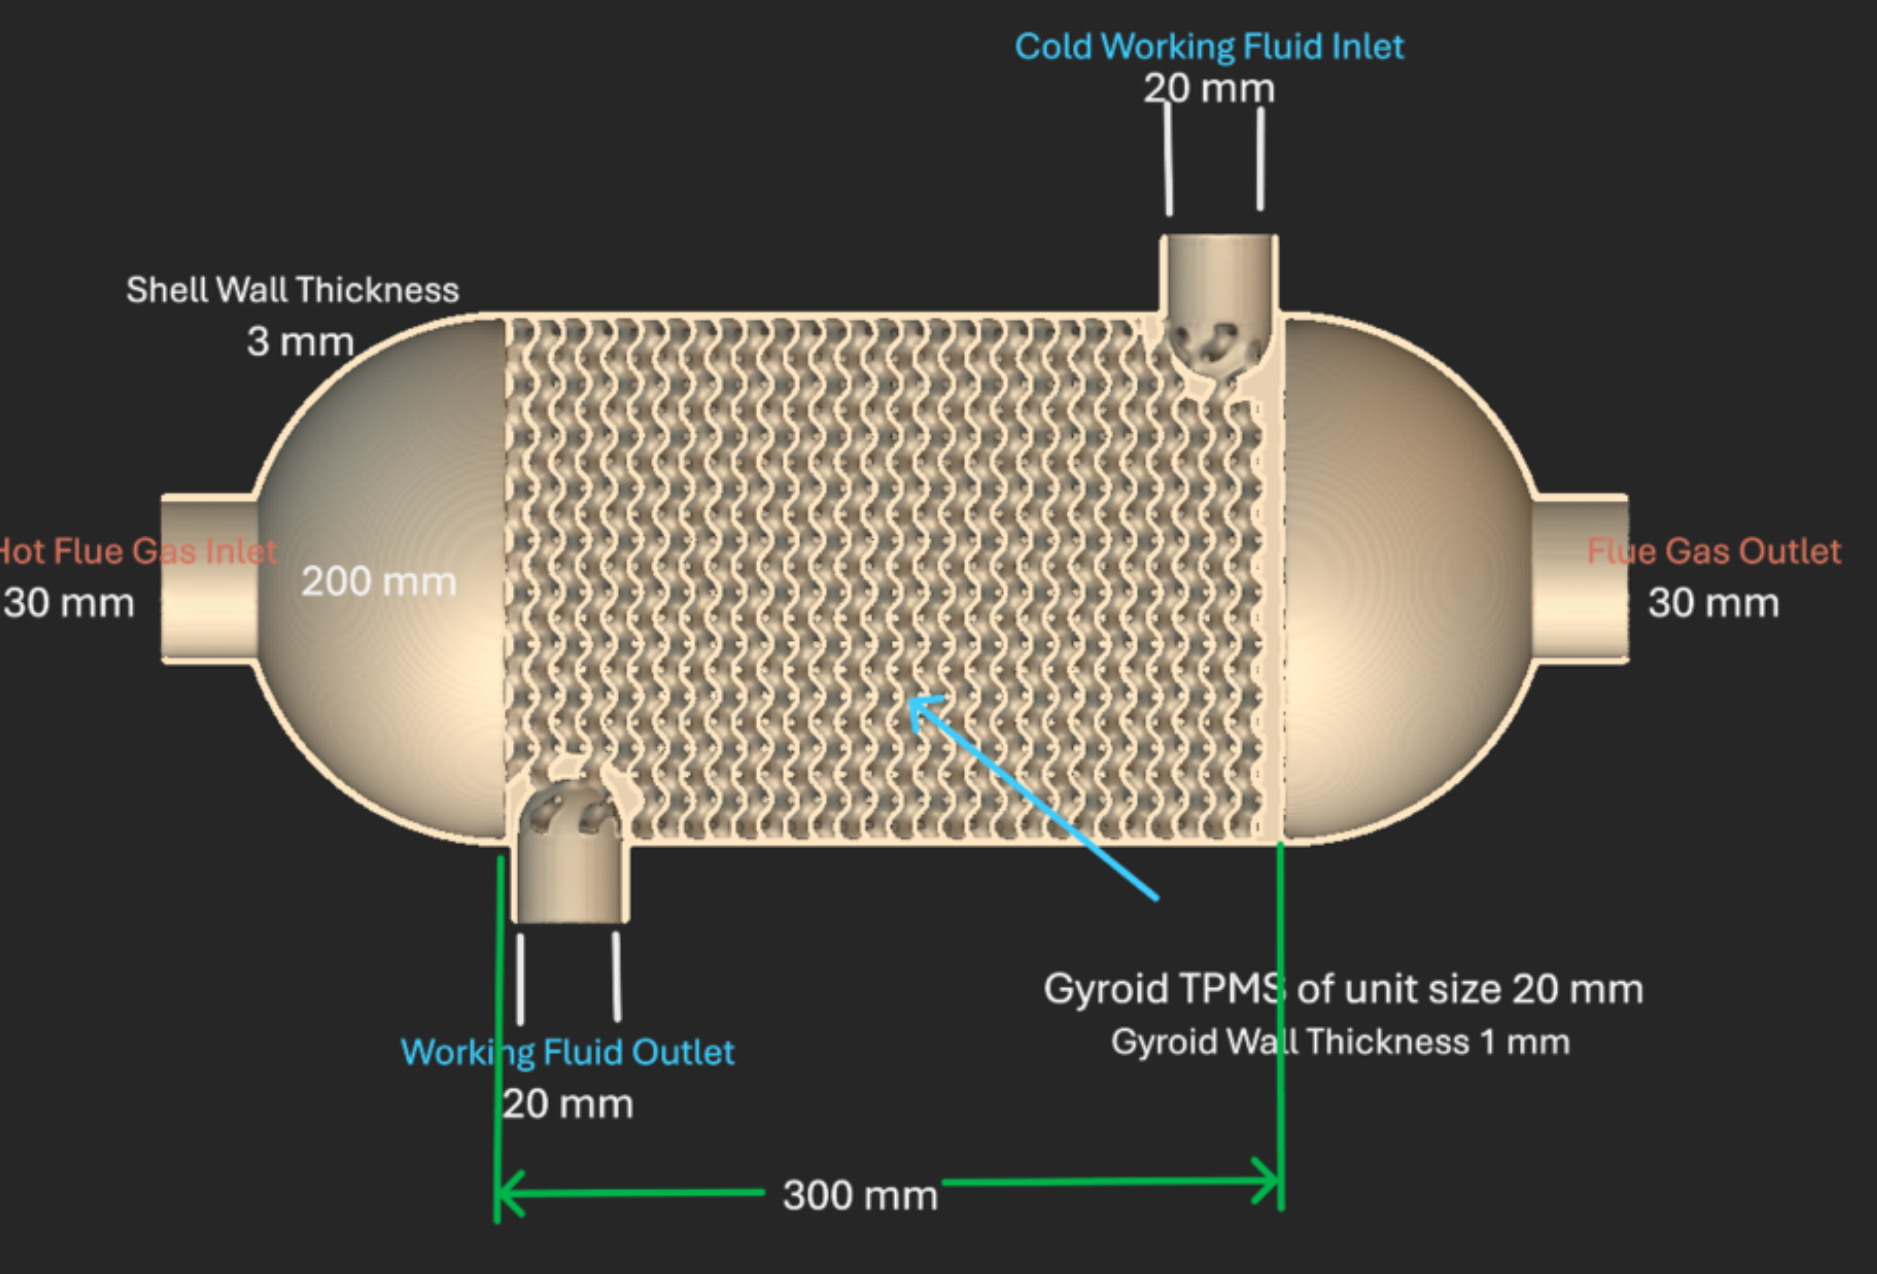
\includegraphics[scale=0.1]{pic/gyroid_exchanger}
	\end{frame}
	
		\begin{frame}{Advantages}
			TPMS provides a compelling alternative to traditional fin-based heat exchangers. 
		\begin{itemize}
			\item High surface-to-volume ratio improves heat exchange.
			\item Continous TPMS walls generally provide good structural integrity (high stiffness).
			\item Geometry can be fine-tuned by function-based parameters. 
		\end{itemize}
	\end{frame}
	
	\begin{frame}{The Problem}
		Dead zones appear in the structure. This causes poor flow utilization, which negatively affects the performance of the heat exchanger. 
		
		\centering
		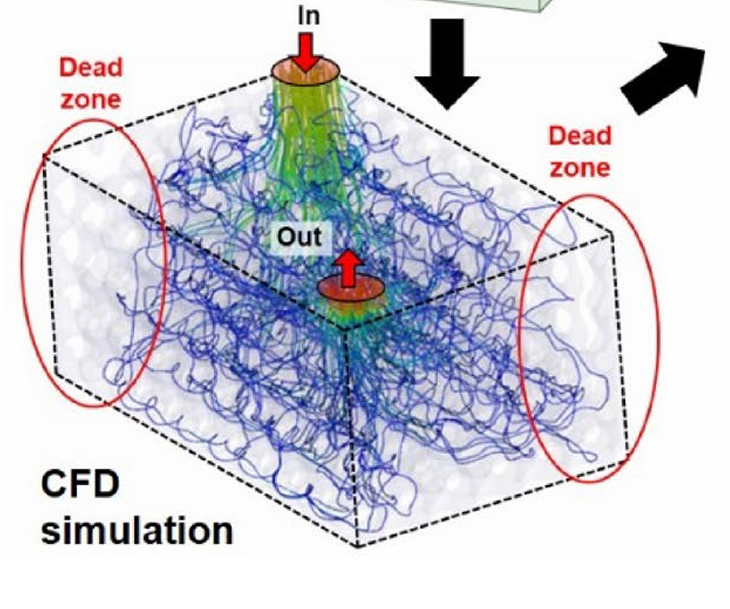
\includegraphics[width=0.4\textwidth]{pic/CFD_dead}
	\end{frame}
	
	\subsection{Numerical simulations}
	\begin{frame}{The Solution: Topology Optimization}
		\centering
		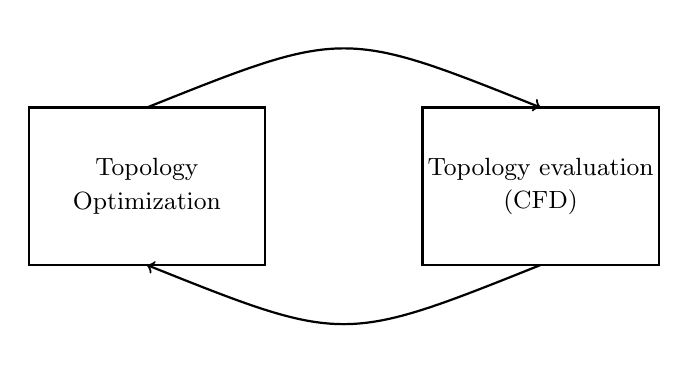
\begin{tikzpicture}
			\draw[thick] (-4,0) rectangle (-1,2) node[pos=0.5, align=center]{\small Topology \\ \small Optimization};
			\draw[thick, ->] (-2.5,2) .. controls (0,3) .. (2.5,2);
			\draw[thick, ->] (2.5,0) .. controls (0,-1) .. (-2.5,0);
			%\draw[thick, ->] (-2.5,2) arc (180:0:2.5);
			%\draw[thick, ->] (2.5,0) arc (0:-180:2.5);
			\draw[thick] (1,0) rectangle (4,2) node[pos=0.5, align=center]{\small Topology evaluation \\ \small (CFD)};
		\end{tikzpicture}
	\end{frame}
		\begin{frame}{The Solution: Topology Optimization}
		\centering
		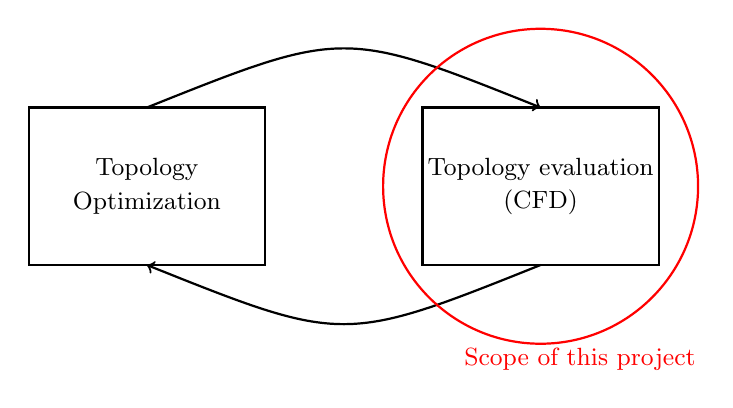
\begin{tikzpicture}
			\draw[thick] (-4,0) rectangle (-1,2) node[pos=0.5, align=center]{\small Topology \\ \small Optimization};
			\draw[thick, ->] (-2.5,2) .. controls (0,3) .. (2.5,2);
			\draw[thick, ->] (2.5,0) .. controls (0,-1) .. (-2.5,0);
			%\draw[thick, ->] (-2.5,2) arc (180:0:2.5);
			%\draw[thick, ->] (2.5,0) arc (0:-180:2.5);
			\draw[thick] (1,0) rectangle (4,2) node[pos=0.5, align=center]{\small Topology evaluation \\ \small (CFD)};
			\draw[red, thick] (2.5, 1) circle (2);
			\node[red] at (3, -1.2) {\small Scope of this project};
		\end{tikzpicture}
	\end{frame}
	\begin{frame}{Current Methods}
		There are several ways to evaluate the performance of a given heat exchanger geometry. 
		\begin{itemize}
			\item \emph{Body-fitted Mesh} is the 'traditional' method which involves meshing of the structure, and evaluation in a FVM framework. 
			\item[-] Well documented but computationally expensive for solving and re-meshing. 
			\pause
			\item \emph{Equivalent porous medium} replaces the TMPS with averaged porous material. 
			\item[-] Very efficient but relatively poor performance \cite{art:porous}
			\pause
			\item \emph{Brinkman penalization} is the method of choice as it can provide sufficient precision in combination with relatively fast results \cite{art:TPMS}. 
		\end{itemize}
	\end{frame}

	\section{Brinkman Penalization}
	\begin{frame}{How it works}



	\begin{itemize}
		\item The solid regions are treated as porous, with permeability $\eta\to 0$ (approaching solid).
		\item A penalty term proportional to the Brinkman force is then added to the Navier-Stokes equation. 
		\item The penalty term is chosen in such a way that the momentum of the fluids approaches zero inside the solid region, making it effectively non-permeable. 
	\end{itemize}
	\end{frame}
	\begin{frame}{Why it works}
		\begin{itemize}
			\item 'Traditional' CFD methods require geometry-specific meshes to be generated. This process can be computationally expensive, especially for complex (read TPMS) geometries. 
			\item During topology optimization, the need to re-mesh the geometry at every iteration renders 'traditional' methods practically unusable for TPMS geometries. 
			\item Methods based on Brinkman penalization mitigate these drawbacks by using only one mesh independent on the specific geometry of the solid region. 
			\item This comes at the cost of lower accuracy, which is acceptable in the early design stage. 
		\end{itemize}
	\end{frame}
	
	\section{Heat Exchanger Physics}
	
	\begin{frame}{How a Heat Exchanger Works}
		A heat exchanger transfers thermal energy between two fluid streams that are kept physically separated.
		\begin{itemize}
			\item A \emph{hot} fluid and a \emph{cold} fluid flow through adjacent channels, separated by a solid.
			\item Heat conducts through the solid wall; convection then distributes it into the bulk of each fluid stream.
		\end{itemize}
	\end{frame}
	
	\begin{frame}{Modeling the Physical Process of Heat Transfer}
		\begin{itemize}
			\item The \emph{flow} in both hot and cold fluids is modeled using momentum and mass conservation. 
			\pause
			\item The \emph{energy} in both hot and cold fluids is modeled using:
		\begin{itemize}
			\item Advection
			\item Diffusion
		\end{itemize}
		\pause
		\item The heat transfer across the solid wall is governed by conduction. 
		\end{itemize}
	\end{frame}
	
\begin{frame}{Heat Transfer Mechanisms}
	Heat is transferred between the two fluid streams via three mechanisms:
	\begin{itemize}
		\item \emph{Conduction} diffuses heat through the solid wall:
		\begin{equation*}
			\mathbf{q}_\text{cond} = -k \nabla T
		\end{equation*}
		\pause
		\item \emph{Advection} carries heat by fluid motion:
		\begin{equation*}
			\mathbf{q}_\text{adv} = \rho c_p T \mathbf{u}
		\end{equation*}
		\pause
		\item \emph{Diffusion} within the fluid also occurs, analogous to the process in the solid:
		\begin{equation*}
			\mathbf{q}_\text{diff} = -k_f \nabla T
		\end{equation*}
	\end{itemize}
\end{frame}

	\begin{frame}{Key Simplifications}
		\begin{itemize}
			\item Steady state; no start-up, transient solutions, or time-dependent conditions.
			\pause
			\item Incompressible flow: density is not varying with temperature or pressure. 
			\pause
			\item All material properties are treated as constant.
			\pause
			\item No turbulent flow. 
			\pause
			\item No viscous dissipation.
			\pause 
			\item No thermal radiation; only convection and conduction. 
			\pause
			\item No thermo-mechanical coupling (no stress/deformation). 
		\end{itemize}
	\end{frame}

	\begin{frame}{The Equations}
		This leads us to the following equations to solve:
		\begin{align*}
			\nabla \cdot u &= 0 \tag{Cont. eqn.} \\
			(u\cdot \nabla)u-\nabla\cdot\frac1{Re}\nabla^2u+\nabla p &=-\alpha u \tag{Momentum eqn. } \\
			u\cdot\nabla T-\nabla\cdot\frac1{Pe}\nabla T &=0 \tag{Energy eqn. }
		\end{align*}
	\end{frame}
	
	
	
	\section{Project Scope}
	
	\begin{frame}{Project Objective}
		Develop a numerical solver for steady-state heat transfer in a gyroid-based 
		heat exchanger using Comsol.
		\begin{itemize}
			\item Solve the coupled flow and heat transfer equations in 3D using
			the Brinkman penalization framework.
			\pause
			\item The gyroid geometry is encoded implicitly through spatially 
			varying penalization and material coefficients.
			\pause
			\item No re-meshing is required when the geometry is modified, 
			consistent with the Brinkman penalization philosophy.
		\end{itemize}
	\end{frame}
	
	\begin{frame}{Why Comsol?}
		\begin{itemize}
			\item Comsol natively supports coupled PDE systems, allowing flow and heat transport 
			to be solved simultaneously within one framework.
			\pause
			\item The Brinkman penalization term can be implemented as a 
			user-defined volume force in the \emph{Laminar Flow} module.
			\pause
			\item Spatially varying material properties can be defined via analytic 
			expressions, directly using the gyroid function.
			\pause
			\item The same mesh is reused across different geometries, making 
			the solver well suited for integration into a topology optimization loop.
		\end{itemize}
	\end{frame}
	
	
	\begin{frame}{Potential Challenges}
		\begin{itemize}
			\item \emph{Numerical stiffness} — the sharp transition in material properties
			at the fluid-solid interface may cause convergence difficulties and 
			a smooth regularization may be needed.
			\pause
			\item \emph{Mesh resolution} — resolving boundary layers near the 
			gyroid wall in 3D is computationally demanding.
			\pause
			\item \emph{Penalization accuracy} — choosing the penalization parameter large enough 
			to enforce no-slip without causing ill-conditioning is a known 
			challenge in Brinkman methods.
			\pause
			\item \emph{Coupling convergence} — the nonlinear coupling between 
			flow and temperature fields may require careful solver tuning 
			in Comsol.
		\end{itemize}
	\end{frame}
	
	
	\section{References}
	
	\begin{frame}[allowframebreaks]
		\bibliography{ref}
		\bibliographystyle{alpha}

	\end{frame}
\end{document}